\clearpage







\section{Abstract}


\subsubsection{One or two sentences providing a basic introduction to the field}
% comprehensible to a scientist in any discipline.



\subsubsection{Two to three sentences of more detailed background}
% comprehensible to scientists in related disciplines.


\subsubsection{One sentence clearly stating the general problem (the gap)}
% being addressed by this particular study.


\subsubsection{One sentence summarising the main result}
%  (with the words “here we show” or their equivalent).


\subsubsection{Two or three sentences explaining what the main result reveals in direct comparison to what was thought to be the case previously}
% or how the main result adds to previous knowledge


\subsubsection{One or two sentences to put the results into a more general context.}



\subsubsection{Two or three sentences to provide a broader perspective, }
% readily comprehensible to a scientist in any discipline.



%%%%%%%%%%%%%%%%%%%%%%%%%%%%%%%%%%%%%%%%%%%%%%%%%%%%%%%%%%%%%%%%%%%%%%%%%%%%%%%%%%%%%%%%%%%%%%%%%%%%%%%%%%%%%%%%%%%%%%%%%%%%%%%%%%%%%%%%%%%%%%%%%%%%%%%%%%%

\clearpage
\section{Introduction}

%%%%%%%%%%%%%%%%%%%%%%%%%%%%%%%%%%%%%%%%%%%%%%%%%%%%%%%%%%%%%%%%%%%%%%%%%%%%%%%%%%%%%%%%%%%%%%%%%%%%%%%%%%%%%%%%%%%%%%%%%%%%%%%%%%%%%%%%%%%%%%%%%%%%%%%%%%%





%%%%%%%%%%%%%%%%%%%%%%%%%%%%%%%%%%%%%%%%%%%%%%%%%%%%%%%%%%%%%%%%%%%%%%%%%%%%%%%%%%%%%%%%%%%%%%%%%%%%%%%%%%%%%%%%%%%%%%%%%%%%%%%%%%%%%%%%%%%%%%%%%%%%%%%%%%%

\clearpage
\section{Methods}

%%%%%%%%%%%%%%%%%%%%%%%%%%%%%%%%%%%%%%%%%%%%%%%%%%%%%%%%%%%%%%%%%%%%%%%%%%%%%%%%%%%%%%%%%%%%%%%%%%%%%%%%%%%%%%%%%%%%%%%%%%%%%%%%%%%%%%%%%%%%%%%%%%%%%%%%%%%

To measure pathogen richness I used data from \cite{luis2013comparison}. 
These simply include known infections of a bat species with a pathogen species. 
Only species with at least one pathogen were included in the analysis.
To control for study bias I collected the number of pubmed and scholar citations for each bat species including synonyms from ITIS \cite{itis} via the taxize package \cite{chamberlain2013taxize}.
The counts were scraped using the rvest package \cite{rvest}.






I used two measures of population structure. 
$F_{ST}$ and the number of subspecies.
The number of of subspecies was counted using the Wilson and Reeder taxonomy \cite{wilson2005mammal}.

\begin{knitrout}\footnotesize
\definecolor{shadecolor}{rgb}{0.137, 0.137, 0.137}\color{fgcolor}\begin{figure}[t]

{\centering 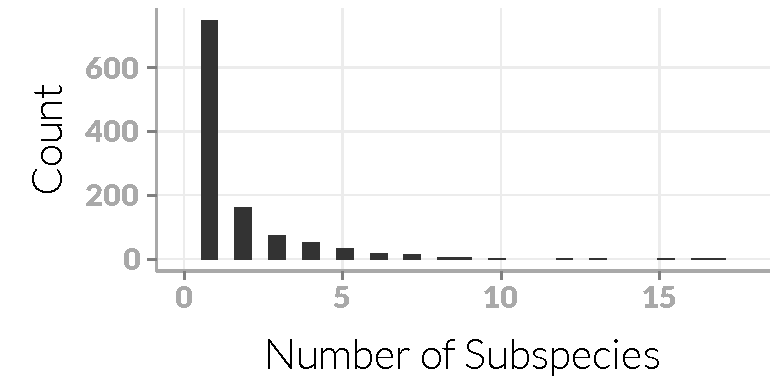
\includegraphics[width=0.8\textwidth]{figure/wilsonReaderTaxonomyRead-1} 

}

\caption[Histogram of number of subspecies]{Histogram of number of subspecies}\label{fig:wilsonReaderTaxonomyRead}
\end{figure}


\end{knitrout}

\begin{knitrout}\footnotesize
\definecolor{shadecolor}{rgb}{0.137, 0.137, 0.137}\color{fgcolor}\begin{figure}[t]

{\centering 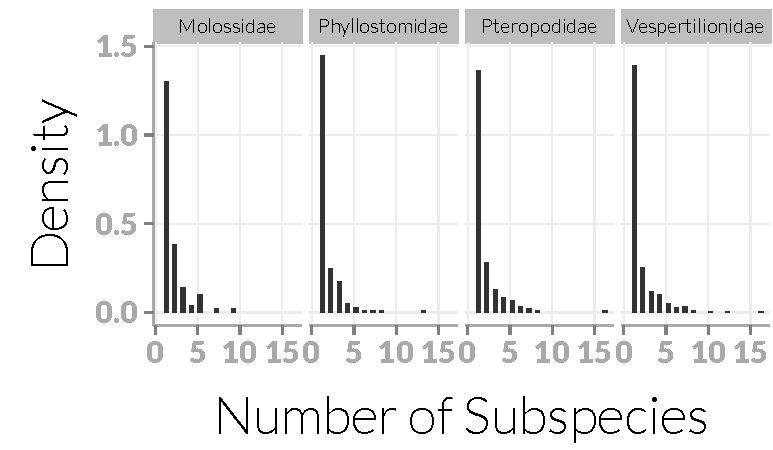
\includegraphics[width=0.8\textwidth]{figure/subsHistsByFam-1} 

}

\caption[Histograms of number of subspecies for the families with many species]{Histograms of number of subspecies for the families with many species.}\label{fig:subsHistsByFam}
\end{figure}


\end{knitrout}



\begin{knitrout}\footnotesize
\definecolor{shadecolor}{rgb}{0.137, 0.137, 0.137}\color{fgcolor}\begin{figure}[t]

{\centering 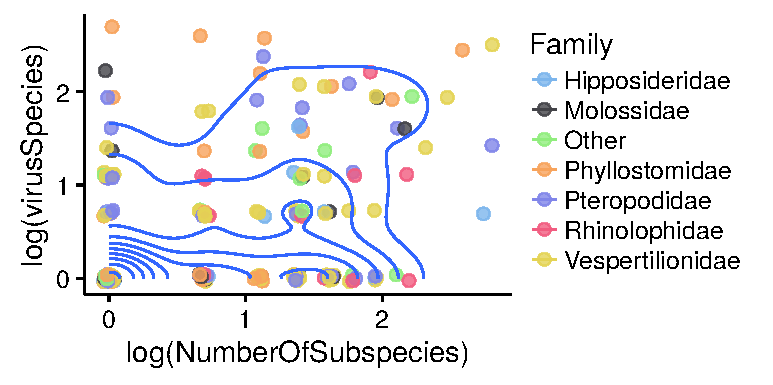
\includegraphics[width=\textwidth]{figure/subsDataFrame-1} 

}

\caption[
Number of viruses against number of subspecies]{
Number of viruses against number of subspecies.
Points are coloured by family, with families with less than 10 species being grouped into "other".
Contours show the 2D density of points and suggest a positive correlation.
}\label{fig:subsDataFrame}
\end{figure}


\end{knitrout}

Measures of bady mass are taken from Pantheria \cite{jones2009pantheria}.












































